\chapter{Develop software development life cycle (SDLC) for Text Classifier.}
\label{Practical:2}
\section{Introduction}
Software Development Life Cycle (SDLC) is a process followed for a software project, within a software organization. It consists of a detailed plan describing how to develop, maintain, replace and alter or enhance specific software. The life cycle defines a methodology for improving the quality of software and the overall development process.\\
SDLC model chosen for the project Text Classifier is Iterative Waterfall Model.Iterative process starts with a simple implementation of a subset of the software requirements and iteratively enhances the evolving versions until the full system is implemented. At each iteration, design modifications are made and new functional capabilities are added. The basic idea behind this method is to develop a system through repeated cycles (iterative) and in smaller portions at a time (incremental).\\
In this incremental model, the whole requirement is divided into various builds. During each iteration, the development module goes through the requirements, design, implementation and testing phases. Each subsequent release of the module adds function to the previous release. The process continues till the complete system is ready as per the requirement.

The key to a successful use of an iterative software development lifecycle is rigorous validation of requirements, and verification & testing of each version of the software against those requirements within each cycle of the model. As the software evolves through successive cycles, tests must be repeated and extended to verify each version of the software.
\section{Advantages of using Iterative waterfall model}
\begin{enumerate}
	\item Some working functionality can be developed quickly and early in the life cycle.
	\item Results are obtained early and periodically.
	\item Parallel development can be planned.
	\item Progress can be measured.
	\item Risk analysis is better.
\end{enumerate}
\section{Phases}
There are six phases in the iterative waterfall model :
\subsection{Requirement analysis and specification}
Requirements for text classifier project are in following fields:
\begin{itemize}
	\item Business: In marketing field companies use it to develop their strategies, to understand customer's feelings towards products or brand, how people respond to their campaigns or product launches and why consumers don’t buy some products.
	\item Politics: In political field, it is used to keep track of political view, to detect consistency and inconsistency between statements and actions at the government level. It can be used to predict election results as well!
	\item Public Actions: Sentiment analysis also is used to monitor and analyse social phenomena, for the spotting of potentially dangerous situations and determining the general mood of the blogosphere.
\end{itemize}
\subsection{Design}
\begin{figure}[H]
	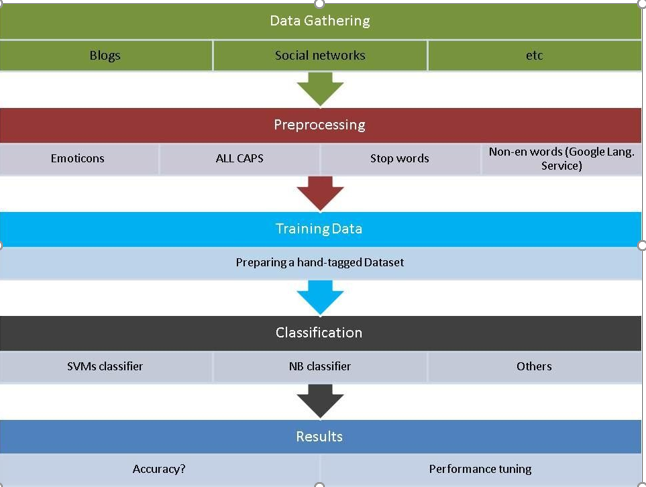
\includegraphics[width=\linewidth]{design.png}
	\caption{Steps involved.}
	\label{fig:boat1}
\end{figure}
First Step: Data Collecting : In this stage data to be analyzed is crawled from various sources like Blogs, Social networks (Twitter, etc.) depending upon the area of application.\\
Second Step: Pre-processing : In this stage, the acquired data is cleaned and made ready for feeding it into the classifier. Cleaning includes extraction of keywords and symbols. For instance – Emoticons are the smiley used in textual form to repre- sent emotions e.g. “:-)”, “:)”, “=)”, “:D”, “:-(“, “:(“, “=(“, “;(“, etc.. Correcting the all uppercase and all lowercase to a common case, removing the non-English (or prof- fered language texts), removing un-necessary white spaces and tabs, etc.\\
Third Step: Training Data : A hand-tagged collection of data is prepared by most commonly used crowd-sourcing method. This data is the fuel for the classifier; it will be fed to the algorithm for learning purpose.\\
Fourth Step: Classification : This is the heart of the whole technique. Depending upon the requirement of the application SVM or Naive bayes is deployed for analysis. The classifier (after completing the training) is ready to be deployed to the real time tweets/text for sentiment extraction purpose.\\
Fifth Step: Results : Results are plotted based on the type of representation selected i.e. charts, graphs, etc. Performance tuning is done prior to the release of the algorithm.

\subsection{Coding and unit testing}
Coding for this project will be done in python.Following python packages need to be installed additionally:
\begin{itemize}
\item Tweepy: tweepy is the python client for the official Twitter API.
\item TextBlob: textblob is the python library for processing textual data.
\end{itemize}
In order to fetch tweets through Twitter API, one needs to register an App through their twitter account and get Consumer Key, Consumer Secret, Access token and Access Token Secret.\\
We'll test this software on our twitter account feed after it is completely developed.
\subsection{Integration and system testing}
Integration testing (sometimes called integration and testing) is the phase in software testing in which individual software modules are combined and tested as a group. It occurs after unit testing and before validation testing. Integration testing takes as its input modules that have been unit tested, groups them in larger aggregates, applies tests defined in an integration test plan to those aggregates, and delivers as its output the integrated system ready for system testing.\\
In text classifier,we will test the same input with various persons manually and their mean value will be compared with the value produced by our software to check it's accuracy and correctness.\\ 
In system testing, we'll conduct test on a complete, integrated system to evaluate the system's compliance with its specified requirements.
\subsection{Maintenance}
In our text classifier project due to change in requirements and conditions,we will take care of following types of maintenances : 
\begin{itemize}
\item Corrective Maintenance : This includes modifications and updations done in order to correct or fix problems, which are either discovered by user or concluded by user error reports.
\item Adaptive Maintenance : This includes modifications and updations applied to keep the software product up-to date and tuned to the ever changing world of technology and business environment.
\item Perfective Maintenance : This includes modifications and updates done in order to keep the software usable over long period of time. It includes new features, new user requirements for refining the software and improve its reliability and performance.
\item Preventive Maintenance : This includes modifications and updations to prevent future problems of the software. It aims to attend problems, which are not significant at this moment but may cause serious issues in future.
\end{itemize}
